\documentclass[a4paper,landscape]{article}
\usepackage{kotex}
\usepackage[margin=12mm]{geometry}
\usepackage{tikz}
\usetikzlibrary{arrows.meta,positioning,fit,calc,backgrounds,shapes.geometric,shadows.blur,matrix}
\usepackage{xcolor}
\usepackage{booktabs}
\usepackage{enumitem}
\usepackage{amsmath}
\usepackage{array}
\usepackage{hyperref}
\hypersetup{colorlinks=true,linkcolor=blue,urlcolor=blue}
\pagestyle{plain}
\setlength{\parindent}{0pt}
\setlength{\parskip}{4pt}

\definecolor{coreblue}{HTML}{2563EB}
\definecolor{corefill}{HTML}{DBEAFE}
\definecolor{programviolet}{HTML}{7C3AED}
\definecolor{programfill}{HTML}{EDE9FE}
\definecolor{policyamber}{HTML}{CA8A04}
\definecolor{policyfill}{HTML}{FEF3C7}
\definecolor{runtimegreen}{HTML}{15803D}
\definecolor{runtimefill}{HTML}{DCFCE7}
\definecolor{dangerred}{HTML}{B91C1C}
\definecolor{dangerfill}{HTML}{FEE2E2}
\definecolor{neutralgray}{HTML}{475569}
\definecolor{neutralfill}{HTML}{F1F5F9}

\tikzset{
  box/.style={draw=neutralgray,rounded corners=2pt,fill=white,align=center,inner sep=5pt,minimum height=9mm,font=\small},
  corebox/.style={box,draw=coreblue,fill=corefill,text=black},
  programbox/.style={box,draw=programviolet,fill=programfill,text=black},
  policybox/.style={box,draw=policyamber,fill=policyfill,text=black},
  runtimebox/.style={box,draw=runtimegreen,fill=runtimefill,text=black},
  dangerbox/.style={box,draw=dangerred,fill=dangerfill,text=black},
  note/.style={draw=neutralgray,rounded corners=2pt,fill=neutralfill,align=left,inner sep=6pt,font=\small},
  flow/.style={-{Latex[length=2.2mm]},line width=0.65pt,draw=neutralgray},
  coreflow/.style={flow,draw=coreblue},
  programflow/.style={flow,draw=programviolet},
  runtimeflow/.style={flow,draw=runtimegreen},
  policyflow/.style={flow,draw=policyamber,dashed},
  forbidden/.style={-{Latex[length=2.2mm]},line width=0.8pt,draw=dangerred,dashed}
}

\begin{document}

\begin{titlepage}
\centering
\vspace*{8mm}
{\Huge\bfseries NeoGraph\par}
\vspace{2mm}
{\LARGE Bounded Self-Evolving Multi-Agent Runtime\par}
\vspace{5mm}
{\large Core DSL, Program DSL, Harness, admission, durable child orchestration, and versioned evolution\par}
\vspace{8mm}
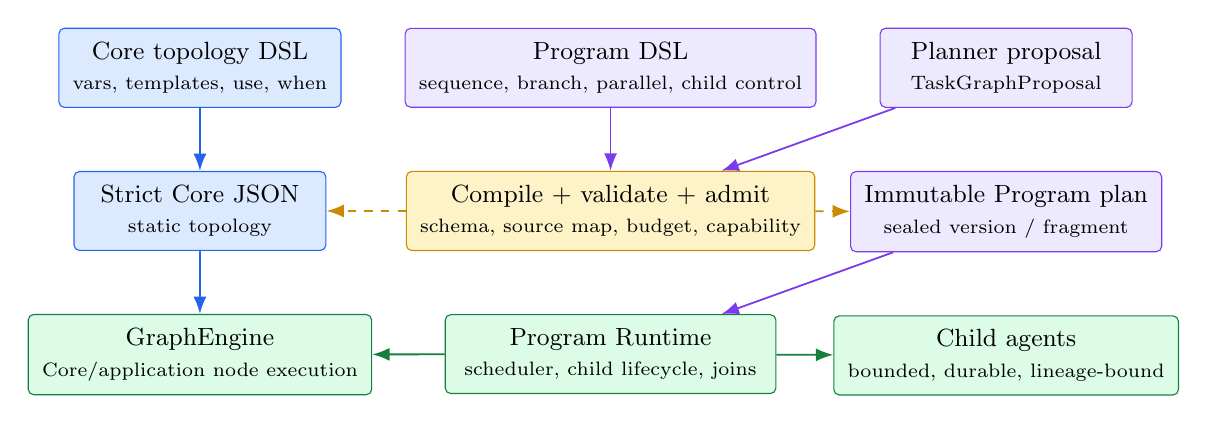
\begin{tikzpicture}[node distance=8mm and 8mm]
  \node[corebox,minimum width=32mm] (coredsl) {Core topology DSL\\{\scriptsize vars, templates, use, when}};
  \node[programbox,minimum width=32mm,right=of coredsl] (programdsl) {Program DSL\\{\scriptsize sequence, branch, parallel, child control}};
  \node[programbox,minimum width=32mm,right=of programdsl] (proposal) {Planner proposal\\{\scriptsize TaskGraphProposal}};
  \node[policybox,minimum width=40mm,below=of programdsl] (compile) {Compile + validate + admit\\{\scriptsize schema, source map, budget, capability}};
  \node[corebox,minimum width=32mm,below=of coredsl] (corejson) {Strict Core JSON\\{\scriptsize static topology}};
  \node[programbox,minimum width=32mm,below=of proposal] (plan) {Immutable Program plan\\{\scriptsize sealed version / fragment}};
  \node[runtimebox,minimum width=42mm,below=of compile] (runtime) {Program Runtime\\{\scriptsize scheduler, child lifecycle, joins}};
  \node[runtimebox,minimum width=32mm,below=of corejson] (engine) {GraphEngine\\{\scriptsize Core/application node execution}};
  \node[runtimebox,minimum width=32mm,below=of plan] (children) {Child agents\\{\scriptsize bounded, durable, lineage-bound}};
  \draw[coreflow] (coredsl) -- (corejson);
  \draw[programflow] (programdsl) -- (compile);
  \draw[programflow] (proposal) -- (compile);
  \draw[policyflow] (compile) -- (corejson);
  \draw[policyflow] (compile) -- (plan);
  \draw[coreflow] (corejson) -- (engine);
  \draw[programflow] (plan) -- (runtime);
  \draw[runtimeflow] (runtime) -- (children);
  \draw[runtimeflow] (runtime) -- (engine);
\end{tikzpicture}
\vfill
\begin{minipage}{0.86\textwidth}
\small\textbf{읽는 법.} NeoGraph는 하나의 통합 DSL이 아니다. Core DSL은 정적 Core topology를 만들고, Program DSL은 sealed Core와 child Program을 유한하게 제어한다. 모델이 제안한 값은 실행 권한이 아니라 검증 대상인 데이터이며, admission을 통과한 immutable version만 실행된다.
\end{minipage}
\vspace{5mm}
{\small 기준 상태: 2026-08-07 \quad Issue \#22 \quad \url{https://github.com/fox1245/NeoGraph-v1-redesign-backup/issues/22}}
\end{titlepage}

\section*{1. 전체 시스템 지도: 두 언어와 하나의 실행 계층}
\begin{tikzpicture}[node distance=9mm and 9mm]
  \node[corebox,minimum width=38mm] (dsl) {Core DSL\\{\scriptsize 정적 확장 언어}};
  \node[corebox,minimum width=38mm,right=of dsl] (elab) {graph::Elaborator\\{\scriptsize finite expansion + source map}};
  \node[corebox,minimum width=40mm,right=of elab] (strict) {Strict Core JSON\\{\scriptsize channels / nodes / edges / barriers}};
  \node[corebox,minimum width=36mm,right=of strict] (graph) {GraphCompiler\\{\scriptsize GraphEngine}};
  \draw[coreflow] (dsl) -- (elab);
  \draw[coreflow] (elab) -- (strict);
  \draw[coreflow] (strict) -- (graph);

  \node[programbox,minimum width=38mm,below=21mm of dsl] (psource) {Program source\\{\scriptsize v1 / v2 / v3 / v4}};
  \node[programbox,minimum width=38mm,right=of psource] (pcompile) {ProgramCompiler\\{\scriptsize normalize + lower}};
  \node[programbox,minimum width=40mm,right=of pcompile] (pplan) {Typed ProgramPlan\\{\scriptsize operation graph + bounds}};
  \node[programbox,minimum width=36mm,right=of pplan] (pruntime) {ProgramRuntime\\{\scriptsize orchestration domain}};
  \draw[programflow] (psource) -- (pcompile);
  \draw[programflow] (pcompile) -- (pplan);
  \draw[programflow] (pplan) -- (pruntime);

  \node[policybox,minimum width=45mm,below=18mm of pcompile] (admit) {Admission boundary\\{\scriptsize registry, owner, tenant, budget, capability, effect}};
  \draw[policyflow] (admit) -- (pcompile);
  \draw[policyflow] (admit) -- (pplan);
  \draw[policyflow] (admit) -- (pruntime);

  \node[runtimebox,minimum width=45mm,below=18mm of pruntime] (durable) {Durable runtime services\\{\scriptsize journal, transition store, checkpoint, host admission}};
  \draw[runtimeflow] (pruntime) -- (durable);
  \draw[runtimeflow] (pruntime) -- (graph);

\end{tikzpicture}

\textbf{의도된 bridge.} Core DSL은 strict Core JSON으로만 내려가고, Program은 그 sealed Core를 \texttt{call\_core}로 호출한다. Core DSL 자체가 Program control VM으로 변하는 것은 아니다.

\textbf{핵심 구분.} Core DSL은 반복 작성과 topology 재사용을 해결한다. Program DSL은 유한한 orchestration과 child lifecycle을 해결한다. 두 언어를 합치지 않는 이유는 Core DSL의 결정성·정적 검증·source map을 보존하기 위해서다.

\begin{center}
\begin{tabular}{p{0.27\textwidth}p{0.27\textwidth}p{0.27\textwidth}}
\toprule
\textbf{Core DSL} & \textbf{Program DSL} & \textbf{Program Runtime} \\
\midrule
vars, interpolation, templates, use, when & sequence, branch, bounded loop/retry, \mbox{parallel}, race, quorum, map, \mbox{parallel\_map}, \mbox{expand\_task\_graph} & spawn, await, cancel, checkpoint, scheduling, joins, recovery \\
static Core topology & typed control tree / task graph & durable execution and authority enforcement \\
\bottomrule
\end{tabular}
\end{center}
\textbf{범례.} \textcolor{coreblue}{파랑} = Core, \textcolor{programviolet}{보라} = Program, \textcolor{policyamber}{황색} = admission/policy, \textcolor{runtimegreen}{초록} = runtime/evidence. 실선은 data/execution flow, 점선은 constraint 또는 authority boundary를 뜻한다.

\newpage
\section*{2. Harness와 외부 authoring 경계}
\begin{tikzpicture}[node distance=8mm and 12mm]
  \node[box,minimum width=34mm] (request) {Harness request};
  \node[corebox,minimum width=36mm,below left=of request] (dslmode) {mode: \texttt{dsl}\\Core DSL definition};
  \node[programbox,minimum width=42mm,below=of request] (programmode) {mode: \texttt{program}\\Program operation tree};
  \node[corebox,minimum width=36mm,below right=of request] (coremode) {mode: \texttt{core}\\strict Core JSON};
  \node[corebox,minimum width=42mm,below=of dslmode] (dslout) {Elaborator\\{\scriptsize Core JSON}};
  \node[programbox,minimum width=42mm,below=of programmode] (progout) {Program compile/admit\\{\scriptsize v2 static; v3/v4 boundary explicit}};
  \node[corebox,minimum width=42mm,below=of coremode] (coreout) {Core validation\\{\scriptsize sealed Core}};
  \node[runtimebox,minimum width=48mm,below=18mm of progout] (run) {Program Runtime\\{\scriptsize one sealed Core + admitted children}};
  \node[dangerbox,minimum width=56mm,right=18mm of request,align=left] (blocked) {\textbf{금지}\\mode=dsl에 Program tree 삽입 금지\\임의 endpoint/credential/executor 금지\\validation 없는 model JSON 실행 금지};
  \draw[flow] (request) -- (dslmode);
  \draw[flow] (request) -- (programmode);
  \draw[flow] (request) -- (coremode);
  \draw[coreflow] (dslmode) -- (dslout);
  \draw[programflow] (programmode) -- (progout);
  \draw[coreflow] (coremode) -- (coreout);
  \draw[programflow] (progout) -- (run);
  \draw[coreflow] (dslout.south) to[bend right=18] (run.west);
  \draw[coreflow] (coreout.south) to[bend left=18] (run.east);
  \draw[forbidden] (dslmode.west) -- ++(-4mm,0) |- (blocked.north west);
\end{tikzpicture}

\textbf{현재 외부 노출의 중요한 사실.} Direct Program API가 v3 \texttt{parallel\_map}과 v4 \texttt{expand\_task\_graph}를 단계적으로 지원하더라도 Harness의 \texttt{program} profile은 별도의 schema/version 계약을 가진다. 따라서 “compiler가 받는다”와 “Harness가 외부에 공개한다”는 동일한 주장이 아니다.

\newpage

\section*{3. Self-evolution과 version swap}
\begin{tikzpicture}[node distance=8mm and 9mm]
  \node[programbox,minimum width=38mm] (proposal) {Planner / agent proposal\\{\scriptsize Core DSL, Program source, TaskGraphProposal}};
  \node[policybox,minimum width=40mm,right=of proposal] (check) {Deterministic checks\\{\scriptsize schema, types, source map, bounds}};
  \node[policybox,minimum width=40mm,right=of check] (admission) {Admission\\{\scriptsize capability, effect, budget, owner, tenant}};
  \node[programbox,minimum width=42mm,below=14mm of admission] (version) {Immutable version\\{\scriptsize Core generation / ProgramVersion / fragment}};
  \node[runtimebox,minimum width=42mm,below=14mm of version] (activation) {Activation / safe point\\{\scriptsize new runs or compatible fork}};
  \node[runtimebox,minimum width=40mm,below left=12mm and 18mm of activation] (oldrun) {Existing run\\{\scriptsize remains pinned to old version}};
  \node[runtimebox,minimum width=40mm,below right=12mm and 18mm of activation] (newrun) {New run\\{\scriptsize starts from new version}};
  \node[dangerbox,text width=42mm,below=13mm of proposal,align=left] (mutate) {\textbf{In-place mutation 아님}\\running GraphEngine을 덮어쓰지 않는다. 새 version을 publish하고 safe point에서만 교체한다.};
  \draw[programflow] (proposal) -- (check);
  \draw[policyflow] (check) -- (admission);
  \draw[policyflow] (admission) -- (version);
  \draw[programflow] (version) -- (activation);
  \draw[runtimeflow] (activation) -- (oldrun);
  \draw[runtimeflow] (activation) -- (newrun);
  \draw[forbidden] (mutate.east) to[bend left=10] (oldrun.west);
\end{tikzpicture}

Self-evolution은 “모델이 원하는 JSON을 실행”하는 것이 아니라 다음의 versioned pipeline이다.

\begin{enumerate}[leftmargin=18mm,itemsep=1pt]
\item proposal은 untrusted data다.
\item compiler가 유한성과 typed contract를 증명한다.
\item admission이 권한·effect·budget을 결정한다.
\item immutable version/fragment가 publish된다.
\item 기존 run은 기존 version에 pin되고, 새 run 또는 safe-point fork만 새 version을 사용한다.
\end{enumerate}

\newpage
\section*{4. 계층형 sub-agent runtime}
\begin{tikzpicture}[x=1mm,y=1mm]
  \node[policybox,minimum width=48mm] (root) at (0,0) {Tenant / root Program\\{\scriptsize global budget + policy + capability}};
  \node[programbox,minimum width=40mm] (sup) at (-55,-20) {Supervisor\\{\scriptsize planner / judge / join}};
  \node[programbox,minimum width=40mm] (review) at (55,-20) {Reviewer panel\\{\scriptsize bounded parallel fan-out}};
  \node[runtimebox,minimum width=36mm] (a) at (-85,-43) {Child A\\{\scriptsize researcher}};
  \node[runtimebox,minimum width=36mm] (b) at (-28,-43) {Child B\\{\scriptsize auditor}};
  \node[runtimebox,minimum width=36mm] (c) at (28,-43) {Child C\\{\scriptsize reviewer}};
  \node[runtimebox,minimum width=36mm] (d) at (85,-43) {Child D\\{\scriptsize verifier}};
  \node[runtimebox,minimum width=36mm] (a1) at (-85,-63) {Grandchild A.1\\{\scriptsize allowed Tool use}};
  \node[runtimebox,minimum width=36mm] (b1) at (-28,-63) {Grandchild B.1\\{\scriptsize bounded subtask}};
  \node[note,text width=48mm,align=left] (limits) at (96,0) {\textbf{Bounded grant}\\depth / children / concurrency\\dynamic compiles / budget / host ceiling\\effective = parent remaining\\교집합: spawn / template / policy};
  \node[note,text width=52mm] (up) at (-60,-82) {\textbf{Dataflow}\\typed input $\rightarrow$ child\\typed artifact $\rightarrow$ join\\evidence/lineage $\rightarrow$ judge};
  \draw[runtimeflow] (root) -- (sup);
  \draw[runtimeflow] (root) -- (review);
  \draw[runtimeflow] (sup) -- (a);
  \draw[runtimeflow] (sup) -- (b);
  \draw[runtimeflow] (review) -- (c);
  \draw[runtimeflow] (review) -- (d);
  \draw[runtimeflow] (a) -- (a1);
  \draw[runtimeflow] (b) -- (b1);
  \draw[policyflow] (root.east) -- (limits.west);
  \draw[programflow] (a1) -- (up);
  \draw[programflow] (b1) -- (up);
\end{tikzpicture}

\textbf{Child가 할 수 있는 일.} 승인된 template의 instance 생성, typed task 수행, host-backed Tool 호출, bounded retry/parallel, 결과 artifact 발행, 위임된 범위의 descendant 생성, await/cancel/checkpoint/recovery가 가능하다.

\textbf{Child가 할 수 없는 일.} arbitrary shell/HTTP/MCP endpoint, credential 생성, executor/provider 임의 선택, capability self-escalation, unbounded recursion, 다른 tenant 상태 접근, live graph mutation은 허용하지 않는다. Tool 권한은 \texttt{can\_use}와 \texttt{can\_delegate}를 분리하며, descendant로 내려갈수록 교집합을 취한다.

\newpage
\section*{5. Repository surface map}
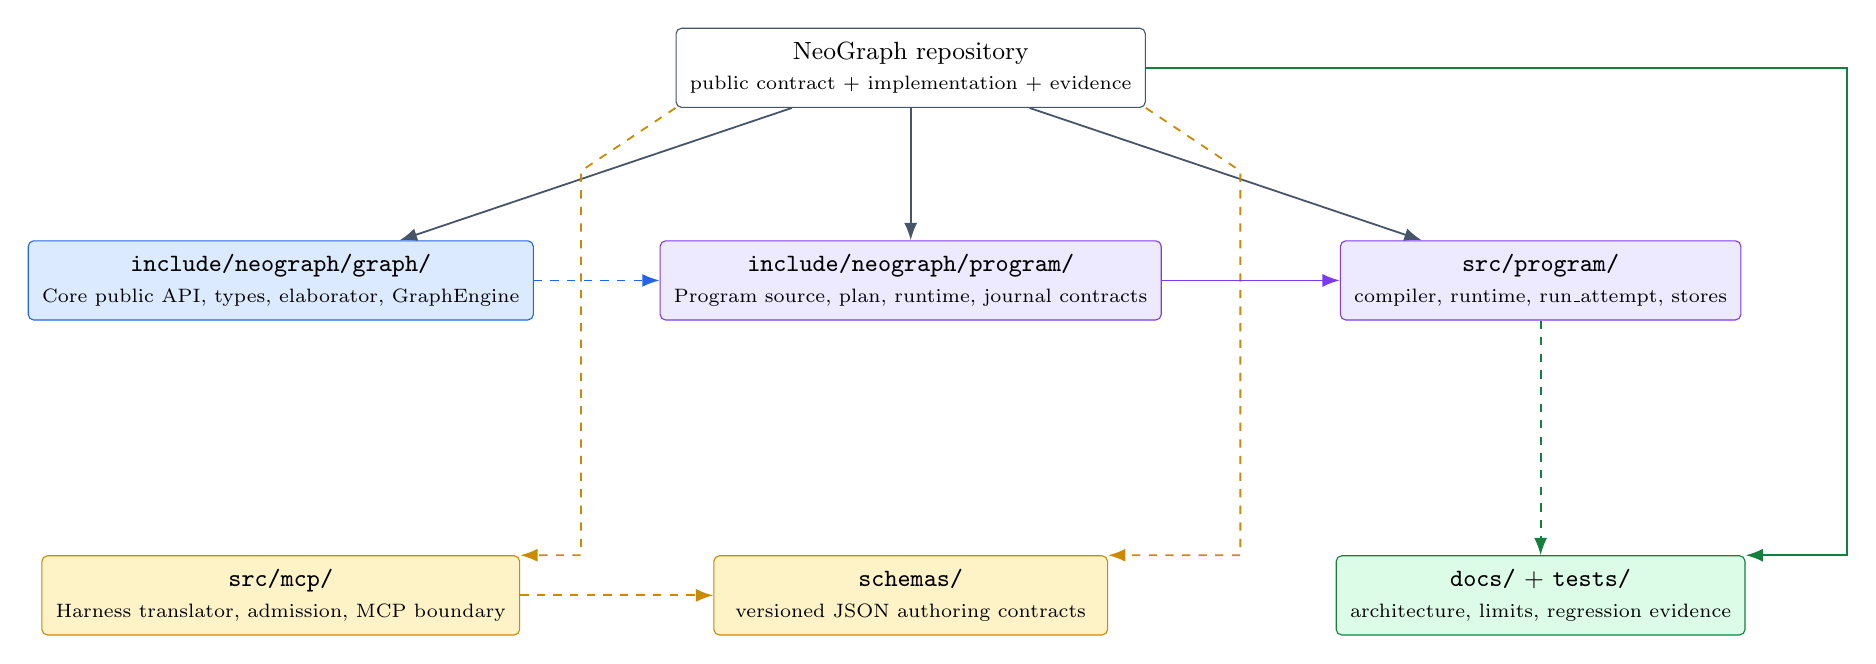
\begin{tikzpicture}[x=1mm,y=1mm]
  \node[box,minimum width=46mm] (repo) at (0,0) {NeoGraph repository\\{\scriptsize public contract + implementation + evidence}};
  \node[corebox,minimum width=50mm] (graphsrc) at (-80,-27) {\texttt{include/neograph/graph/}\\{\scriptsize Core public API, types, elaborator, GraphEngine}};
  \node[programbox,minimum width=50mm] (programinc) at (0,-27) {\texttt{include/neograph/program/}\\{\scriptsize Program source, plan, runtime, journal contracts}};
  \node[programbox,minimum width=50mm] (programsrc) at (80,-27) {\texttt{src/program/}\\{\scriptsize compiler, runtime, run\_attempt, stores}};
  \node[policybox,minimum width=50mm] (mcpsrc) at (-80,-67) {\texttt{src/mcp/}\\{\scriptsize Harness translator, admission, MCP boundary}};
  \node[policybox,minimum width=50mm] (schemas) at (0,-67) {\texttt{schemas/}\\{\scriptsize versioned JSON authoring contracts}};
  \node[runtimebox,minimum width=50mm] (evidence) at (80,-67) {\texttt{docs/} + \texttt{tests/}\\{\scriptsize architecture, limits, regression evidence}};
  \draw[flow] (repo) -- (graphsrc);
  \draw[flow] (repo) -- (programinc);
  \draw[flow] (repo) -- (programsrc);
  \draw[policyflow,dashed] (repo.south west) -- ++(-12mm,-8mm) |- (mcpsrc.north east);
  \draw[policyflow,dashed] (repo.south east) -- ++(12mm,-8mm) |- (schemas.north east);
  \draw[runtimeflow] (repo.east) -- ++(89mm,0) |- (evidence.north east);
  \draw[coreflow,dashed] (graphsrc) -- (programinc);
  \draw[programflow] (programinc) -- (programsrc);
  \draw[policyflow,dashed] (mcpsrc) -- (schemas);
  \draw[runtimeflow,dashed] (programsrc) -- (evidence);
\end{tikzpicture}

\textbf{Repository를 읽는 순서.} 먼저 \texttt{include/}에서 public contract를 보고, \texttt{src/}에서 compiler/runtime/Harness 구현을 확인한다. 그 다음 \texttt{schemas/}에서 외부 authoring 계약을, \texttt{docs/}와 \texttt{tests/}에서 의도와 회귀 증거를 대조한다.

\begin{center}
\begin{tabular}{p{0.29\textwidth}p{0.29\textwidth}p{0.29\textwidth}}
\toprule
\textbf{Public contract} & \textbf{Implementation} & \textbf{Boundary and evidence} \\
\midrule
\texttt{include/neograph/graph/}\newline Core surface &
\texttt{src/program/}\newline compiler, runtime, stores &
\texttt{schemas/}\newline versioned JSON contracts \\
\texttt{include/neograph/program/}\newline Program surface &
\texttt{src/mcp/}\newline Harness integration &
\texttt{docs/} + \texttt{tests/}\newline architecture, limits, regression evidence \\
\bottomrule
\end{tabular}
\end{center}

\newpage
\section*{6. Delivery map과 현재 상태}
\begin{tikzpicture}[x=3.3cm,y=1cm]
  \draw[flow] (0,0) -- (5.5,0);
  \node[box,draw=runtimegreen,fill=white,text width=30mm,minimum height=17mm] at (0,0.55) {\textbf{P0}\\{\scriptsize Contract / IR}};
  \node[box,draw=runtimegreen,fill=white,text width=30mm,minimum height=17mm] at (1.1,0.55) {\textbf{P1}\\{\scriptsize Static Program}};
  \node[box,draw=runtimegreen,fill=white,text width=30mm,minimum height=17mm] at (2.2,0.55) {\textbf{P2}\\{\scriptsize parallel\_map}};
  \node[box,draw=policyamber,fill=white,text width=30mm,minimum height=17mm] at (3.3,0.55) {\textbf{P3}\\{\scriptsize expand\_task\_graph}};
  \node[box,draw=neutralgray,fill=white,text width=30mm,minimum height=17mm] at (4.4,0.55) {\textbf{P4}\\{\scriptsize Durable hierarchy}};
  \node[box,draw=neutralgray,fill=white,text width=30mm,minimum height=17mm] at (5.5,0.55) {\textbf{P5}\\{\scriptsize Evaluation}};
  \node[note,text width=60mm,below=13mm] at (1.0,-0.8) {\textbf{완료}\\P0 TaskGraphProposal IR, P1 static Program surface, P2 bounded parallel\_map};
  \node[note,text width=60mm,below=13mm] at (3.3,-0.8) {\textbf{진행}\\P3는 schema/compiler/typed plan과 runtime publication/dispatch/recovery를 연결해야 한다.};
  \node[note,text width=60mm,below=13mm] at (5.55,-0.8) {\textbf{예정}\\P4 N-level durable hierarchy, P5 single-agent baseline과 비용/효용 평가};
\end{tikzpicture}

\vspace{7mm}
\begin{center}
\begin{tabular}{p{0.30\textwidth}p{0.30\textwidth}p{0.30\textwidth}}
\toprule
\textbf{지금 안정적으로 가능한 것} & \textbf{아직 조심해야 하는 것} & \textbf{P5 이후에도 비목표} \\
\midrule
정적 Core topology 생성, 유한 static Program, 직접 Program API의 bounded parallel\_map, sealed template 기반 작업 & Harness에서 최신 v3/v4 dynamic surface 공개, v4 runtime publication, N-level recovery, 대규모 fairness/throughput & arbitrary code/endpoint/credential, 무제한 recursion, in-place mutation, 다중 agent의 자동 진실 보장 \\
\bottomrule
\end{tabular}
\end{center}

\section*{설명: 이 리포를 이해하는 순서}
\begin{enumerate}[leftmargin=18mm,itemsep=2pt]
\item 먼저 Core DSL과 Program DSL을 분리해서 본다. Core DSL은 graph를 만들고 Program DSL은 graph/child를 제어한다.
\item 그 다음 admission을 본다. 모델이 제안한 JSON은 실행 권한이 아니며, template·Tool·budget·tenant policy의 교집합을 통과해야 한다.
\item 그 다음 runtime을 본다. ProgramRuntime은 GraphEngine을 대체하지 않고, child lifecycle·join·budget·recovery를 담당하는 별도 scheduling domain이다.
\item 마지막으로 self-evolution을 본다. evolution은 live mutation이 아니라 새 immutable version을 만들고 activation/safe point에서 교체하는 과정이다.
\end{enumerate}

\vfill
\begin{center}\small\textit{이 문서는 현재 설계와 보고된 P0--P2 완료 상태, P3 진행 경계를 시각화한 architecture map이다. 구현이 변경되면 상태 페이지와 operation/version 표를 함께 갱신해야 한다.}\end{center}

\end{document}
